% !TEX root = thesis.tex
\chapter{深層学習の実装における技術}
この章では、深層学習のアルゴリズムを実装して、実際の問題に適用するに当たって、どのようにすれば良い結果が得られるか、紹介する。
\section{評価基準}
深層学習のアルゴリズムを使用するための具体的な手段を選ぶにあたり、次のような判断基準を設けた。優先順位は、1→2→3の順に高い。
基準1. 深層学習が注目された大きな理由である、高い識別精度を再現できる。
基準2. 学習にかかる時間が、他のアルゴリズムに比べて、極端に長くならない。
基準3. 利用にあたって必要なプログラミング量が出来るだけ少なく、バグが混入しにくい。
基準1は最優先目標である。今回深層学習を選択した理由は、ウェブ工学のタスクにおいて、高い分類精度を実現するための最も有力な方法だと思われるからである。つまり、例え深層学習のアルゴリズムとして正しいプログラムだったとしても、分類精度が従来の分類器より劣っていれば意味はない。従来の分類器をそのまま使い続ければよいことになってしまう。
基準2と3は、現実の問題を深層学習で解決する際に、必要となってくる視点である。プログラムの作成や、学習の実行にかかる時間が、あまりにも長くなってしまうと、実際のビジネスや、刻一刻と変化するウェブサービスに対して応用するのは非現実的だろう。
\section{既存ソースコード使用の利点}
深層学習のプログラムを実行するために、まず大きく分けて、「自分でソースコードを全て書く」方法と、「主に既存のソースコードを利用する」方法の2つが考えられる。今回は、既存ソースコードをベースに使うことを選択した。以下、その理由を説明する(図\ref{c4_library_merit}参考)。\par
「既存のソースコードを利用する」場合のメリットとして、「開発期間は基本的にゼロで済む」「新たにバグが混入する危険性が無い」「自分の改造コードが、他のライブラリ利用者によって使ってもらえるチャンスが大きい」という点が挙げられる。デメリットとして、「ソースコード中にブラックボックスが増え、改造にかかる時間が短くなる」「全く新しいアルゴリズムを実装する場合、ゼロからスタートした方が早く書けるケースもある」などが想定される。しかし、基準3の「プログラミング量が少なくバグのリスクが低い」という点において優れているため、今回は既存のソースコードを探して利用していくことにした。既存ソースコードを利用する際に生じるリスクについては、図\ref{c4_library_hedge}のように対処できる。\par

\begin{figure}[tbp]
 \begin{center}
  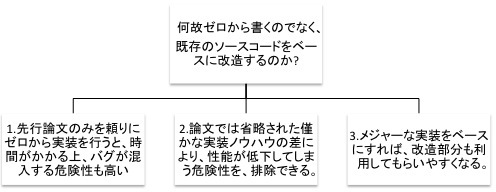
\includegraphics[width=100mm]{img/c4/library_merit}
 \end{center}
 \caption{既存コードの利用における、完全オリジナルコードの作成に対する利点}
 \label{c4_library_merit}
\end{figure}

\begin{figure}[tbp]
 \begin{center}
  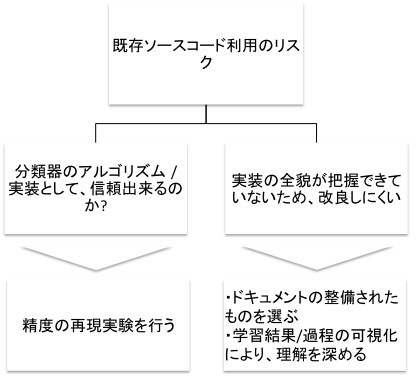
\includegraphics[width=120mm]{img/c4/library_hedge}
 \end{center}
 \caption{既存ソースコード利用のリスクと、対処方法}
 \label{c4_library_hedge}
\end{figure}

なお、「自分でソースコードを全て書く」場合のメリットとデメリットは、上記「既存のソースコード」の場合の逆となる。自分で新たなコードを書くので時間がかかり、バグの混入リスクも大きい。また、ソースコードを公開した場合の、ライブラリとしての信頼度も、ゼロから築かなければならない。ただし、コードの詳細部分を改造する段階では、自分の手で書いたコードを使う方が、より深い理解を得やすく、確実で素早い実装ができる可能性もある。\par

\section{グラフィックスプロセッシングユニットの利用による高速化}
現代のGPUは、単にグラフィック処理に特化したプロセッサというだけでなく、その並列演算能力を活かして、大量の演算を行う科学計算用途にも使われている。GPU設計・製作メーカーのNVIDIAからは、グラフィック出力機能を敢えて外し、科学計算用途に特化した、TeslaというハイエンドGPUシリーズも発売されている\footnote{\url{http://www.nvidia.co.jp/object/tesla-supercomputing-solutions-jp.html}}。\par 
深層学習の研究においても、GPUによる並列計算が有効とされている。これは、入力ベクトルと重み行列の積など、ニューラルネットワークの計算にて中心を占める行列演算が、並列計算の恩恵を受けやすいからである\cite{bengio2012practical}。例えば、Dropconnectの研究に拠れば、GPUで演算した場合、テクスチャメモリを利用しなくてもCPUより97.2倍高速化でき、テクスチャメモリを利用すれば414.8倍の速度を出すことも可能である\cite{wan2013regularization}。\par
また、深層学習の実装によっては、はじめからGPUで高速化することを前提に、GPU専用のコードを書いている場合がある。例えば、後述するcuda-convnet\footnote{\url{https://code.google.com/p/cuda-convnet/}}や、Maxout Network\cite{goodfellow2013maxout}のコードの一部、DropConnect\cite{wan2013regularization}\footnote{\url{http://cs.nyu.edu/~wanli/dropc/}}が該当する。この場合、そもそもGPUを搭載したマシンを使わないと、コンパイルや実行が全く出来なくなってしまう。\par
%CPUの計算能力は頭打ちになっている。
GPUが高速に演算を実行できる理由は、その構造にある。1〜数個のプロセッサで様々な命令をこなすCPUに対し、GPUは数百〜数千個のcoreを持っており、同一の命令を高速に並列演算する用途に向いている。これは、大量の点の変換処理が必要となるグラフィック処理環境から生まれたGPUの強みである。かつてGPUを科学演算に用いるには、OpenGLやCgのようなグラフィック処理用ライブラリを使ってアルゴリズムを記述しなくてはならず、非常に難易度が高かった\footnote{\url{http://www.nvidia.co.jp/object/what-is-gpu-computing-jp.html}}。そこで、NVIDIAはCUDAというGPUによる演算の開発環境を開発した\cite{garland2008parallel}。CUDAはC/C++言語を拡張した作りになっており、グラフィックライブラリに比べて記述は非常に容易である。また、PythonにてCUDAコードを生成するライブラリも存在している\cite{klockner2009pycuda:}\cite{klockner2012pycuda}。\par
GPUによる並列演算は高速だが、GPUのメモリとCPUのメモリとの間で起こる通信は、比較して低速であり、ボトルネックになることが多い。通信の回数を減らし、GPU上のみで完結する演算を増やすことが重要である\cite{bengio2012practical}。


\section{深層学習のライブラリ}
深層学習に利用できるライブラリは、まだ標準が固まっていないものの、論文と共にソースコードを公開するパターンが多く、いくつか出回っている。この節では、深層学習関係のライブラリやソースコードを紹介する。

\subsection{cuda-convnet}
CUDAとC++による畳み込みネットワークの実装が、CIFARデータセットの制作者であるKrizhevsky氏によって公開されている\footnote{\url{https://code.google.com/p/cuda-convnet/}}。最大値蓄積 レイヤーや最終レイヤー用のソフトマックス レイヤーなど、畳み込みネットワークの実装に必要なパーツが一通り用意されている。なお、後述するPylearn2にも、このcuda-convnetのPythonラッパクラスが実装されている。

\subsection{word2vec}
何度か触れてきたが、word2vecのコードも全て公開されており、誰でもテキストデータを入れて、意味ベクトルを生成できるようになっている\footnote{\url{https://code.google.com/p/word2vec/}}。word2vecは、入力されたテキストデータから、まず単語の辞書を作り、次にそれぞれの単語の意味をベクトル化していく。ベクトル化が済めば、単語同士の類似度を計測したり、クラスタリングに用いることができる。

%\subsection{Dropconnect}
%Dropconnectのソースコードも、ウェブページにて公開されている。CUDAとC++を用いた独自のコード

\subsection{数値計算ライブラリTheano}
Theanoは、python上で記述される数式処理/数値計算ライブラリである。Theanoは、数式のコンパイルと実際のデータによる数値計算の2段階で動作する\cite{bergstra+al:2010-Scipy}。図\ref{c4_Theano_compile}に、Theanoが動作する仕組みを示した。
\begin{figure}[tbp]
 \centering
  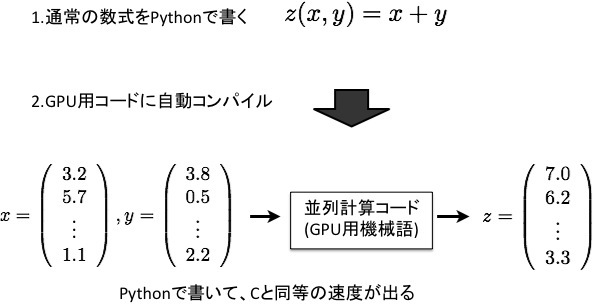
\includegraphics[width=100mm]{img/c4/theano_compile}
 \caption{Theanoの動作過程}
 \label{c4_Theano_compile}
\end{figure}
Theanoでは、数式は文字シンボルを用いた文字式で記述できる。記述された文字式は、内部的には計算木(グラフ)として蓄積されている。Theanoは、実際の計算を行う前に、このグラフをコンパイルして、CによるCUDAのコードに変換している。このときデバッグの難しい数値計算の誤差絡みの部分、0による除算など危険な処理を、自動的に解析してくれる。ニューラルネットワークの演算過程では、非常に小さい数値が出現することがあり、また、文字式を分析することで、計算グラフも最適化してくれる。プログラマは、プログラム上の些末な計算テクニックに囚われることなく、数式の本質的な部分の記述に集中することができる。また、微分も自動で行ってくれる。ニューラルネットワークでは、様々な文字の微分が必要になり、多層にすると爆発的に式が複雑になる。これを手計算による文字式の微分をしてから書いていくと、層を増やす度に手計算が必要になり、非常に煩雑で、開発効率が落ちてしまう。Theanoの自動微分と自動最適化は、Pylearn2の内部記述の簡略化を大いに助けているおいて、多層のニューラルネットワークを使うときでも、文字式に対する大量の手計算と、大量のプログラムの式を書くことなく、簡単に微分やニューラルネットワークを拡張することができる。
\subsection{Deep Learning Tutorial}
Deep Learning Tutorialは、Theanoを用いて記述されたソースコードで、Theanoと同じくLISA.研究室のメンバーによって書かれている。内容的には、単純なロジスティック回帰から始まり、最終的に畳み込みネットワーク, 積層雑音除去自己符号器, 深層信念ネットワークの3つの原理が理解できるよう構成されている。ソースコードのほぽ全ての部分に、詳細なコメントが書いてあり、深層学習のアルゴリズムと同時にTheanoを用いた実装上の注意点なども理解できるような作りになっている。\par
一方で、提供されているコードは簡単のため、アルゴリズムの基本的な部分に絞られており、最新の研究成果が反映されているわけではないため、注意が必要である。例えば、畳み込みネットワークのソースコードには、1998年のLeCunらによる研究\cite{lecun1998gradient-based}をベースにしていると書いてある。しかし、元の論文の段階で既に、2012年に発表された最も優れている畳み込みニューラルネットワーク\cite{ciresan2012multi-column}に比べて、3倍以上誤差が大きくなってしまっている。またあくまでTutorialという位置づけのため、繰り返し回数などのハイパーパラメータが最も誤差が低くなるようには設定されていない。\par
なお、深い構造の形にはなっていないが、雑音除去自己符号器の代わりとして、契約自己符号器\cite{rifai2011contractive}\cite{rifai2011learning}の実装も提供されている。これは、雑音除去自己符号器の亜種だが、誤差測定時に適切なベナルティ項を与えることで、学習される表現の頑健性がさらに向上するというものである。

\subsection{機械学習ライブラリPylearn2}
Pylearn2は、pythonで記述された、深層学習など機械学習アルゴリズムを使うためのライブラリである\cite{goodfellow2013Pylearn2:}。モントリオール大学のLISA.研究室の方がメインとなって、github上で現在も開発が続けられている。LISA.研究室を中心とする開発者によって、ソースコードの開発がほぼ毎日行われている。以下、Pylearn2の長所を記す。
\subsubsection{高精度アルゴリズムMaxout Networkの実装}
Pylearn2には、3章にて述べた、Maxout Networkという深層学習のアルゴリズムの一種が実装されている。このアルゴリズムは、画像認識タスクにおいて非常に高い精度を実現しており、基準1を満たす上で都合が良い。
\subsubsection{Theanoの利用}
Pylearn2のプログラムは、前述したTheanoを全面的に利用して記述されている。Theanoを用いたことで、可読性が大きく上昇している。
\subsubsection{高度な拡張性と可読性}
Pylearn2のソースコードは、拡張性や可読性を非常に強く意識して書かれている。基本的な使い方を記したチュートリアルのウェブページが存在し、主なソースファイルには、詳細なドキュメントも記述されている。また、モジュール化が丁寧なので、自分で書く部分が少なくて済む。例えば、データセットを変更する場合は、Datasetクラスのみを書き下せばよく、他の部分に対してコードを書く必要がほとんどない。図\ref{c4_Pylearn2_yaml}に、Pylearn2において機械学習のアルゴリズムがどのようにモジュール化されているかを示す。\par
また、プログラムを改造する場合でも、数値パラメータを変更するだけであれば、設定ファイルのみの変更で完結させることができる。この設定ファイルは、YAML(YAML Ain't a Markup Language)形式に少し独自拡張を加えた形式になっている。\par
プログラム本体と、数値の設定ファイルが分離されていることで、プログラミングが不得手な人でも、比較的簡単に設定を変更することができる。\par
\begin{figure}[tbp]
 \begin{center}
  \includegraphics[width=80mm]{img/c4/Pylearn2_yaml}
 \end{center}
 \caption{Pylearn2の実験計画例}
 \label{c4_Pylearn2_yaml}
\end{figure}

\subsubsection{Pylearn2の主なパッケージ}
現在のPylearn2のソースコードは、使われているものと非推奨のものが混在している。これは、Pylearn2に定められたAPI変更のルールのためである。Pylearn2では、「変数やクラスを消去する半年前に、ライブラリ上で告知しなければならない」という管理方針を定めている。これは、Pylearn2の安定性に寄与しているが、一方で、ソースコードリーディングの際には使われていないパッケージがノイズになることも少なくない。ここでは、Pylearn2で現在使われている主なパッケージについて紹介する。
\begin{itemize}
\item \textbf{costs} 最終レイヤーで誤差を計算するときに使われる、損失関数(loss function)を集めたパッケージである。主にSGDによって利用される。Dropout、Lpペナルティ、クロスエントロピー関数、負の対数尤度関数などがここに含まれている。また、DBNや自己符号器のように、独自の損失関数が必要な場合も、ここで定義されている。
\item \textbf{datasets} MNISTやCIFAR10, SVHNなどのデータセットがクラス化されている。新しいデータセットに対して深層学習を使いたい場合は、ここに定義されているDatasetクラスやDenseDesignMatrixクラスのサブクラスを作成することになる。
\item \textbf{distributions} ガウス分布などの分布関数が集められている。
\item \textbf{gui} 主に重みフィルタを可視化するためのクラスが用意されている。
\item \textbf{linear} Theanoの線形変換クラスを作り直したもので、畳み込みレイヤーもここに含まれる。
\item \textbf{models} 自己符号器、RBMなどの学習モデルが定義されている。
\item \textbf{sandbox} cuda-convnetのラッパクラスが定義されている。
\item \textbf{scripts} 実際に学習を行わせたり、学習結果を集計するときに便利なスクリプトが集められている。
%\item \textbf{train_extensions} 学習がスタートする時や、1回の処理が終了したときに動かす処理を定義するための、Observerクラスである。
%\item \textbf{training_algorithms} SGDとバッチ勾配降下法を始めとする、学習アルゴリズムが定義されている。SGDと併用するための、学習率変化(線形減少、指数関数的減少、焼き鈍し)、慣性率、Polyak averagingなども、ここで一緒に定義されている。


\end{itemize}

\section{ハードウェアの構成}
深層学習に限った話ではないが、機械学習のタスクは長時間の計算を必要とする場合が多く、プログラムの実行時間が1日以上かかることも稀ではない。普段使用しているPCが使えなくなると困る場合は、機械学習を動かしておくための専用サーバを用意することが望ましい。\par
GPUは必ずしも搭載していなくとも良いのだが、実践上TheanoやCUDAの性能を最大限に生かすためには、GPUを搭載しなければならない。また、CUDAを用いてGPUマシン専用に書かれたアルゴリズムを動作させるためには、GPUが必須となる。GPUは、NVIDIA製で、CUDAに対応していなければならない。ただし、グラフィック出力の機能はなくても構わない。2013年1月現在、NVIDIAのウェブページに掲載されているGPUに関しては、全てCUDAに対応しているため、店舗で新品のGPUを購入する場合は基本的に問題は生じないと思われる。\par
NVIDIAのGPUの中で、どれを選ぶかも問題になる。NVIDIAのウェブページでは、GPUのうちTeslaというシリーズがGPGPUに特化しており、非常に高精度/高速な演算を行うことができる、と述べられている。しかし、非常に高価な上、Teslaシリーズは一般的なグラフィックカードではなく、サーバ全体の購入を基本としている。販売員の方によれば、Teslaは主に商用の大規模データや、ミスの許されない長時間科学計算などに用いることを想定して作られている。今回の目的は、ウェブ工学の一般的タスクにおける深層学習技術を確立するという、いわば実験的な用途であり、Teslaの利用はオーバースペックだと思われる。\par
NVIDIAのGPUは、Teslaを除くと、QuadroとGeForceという2つのシリーズに分かれている。店舗の販売員の方に詳しい話を伺ったところ、Quadroはコンピュータグラフィックの出力機能に注力したシリーズであり、GeForceはより計算性能重視という傾向をもっている。つまり、深層学習の計算などGPGPUに用いる場合、同じ価格帯ならば、GeForceシリーズのGPUを用いた方が、費用対効果が大きくなると考えられる。\par
また、販売員の方によれば、GeForceシリーズの中でもTitanという機種は、Tesla用の部品の中で品質チェックに漏れてしまったものを流用しており、Teslaとほぼ同様の、非常に高い性能を発揮することが出来る、とのことだった。しかし、今回利用する中で最も計算量が大きいMaxout Networkについて、元の発表論文によれば、GeForceシリーズのGTX 580という、少し世代が前のGPUが用いられている。深層学習を実行させる上で、GPUが存在すること自体は非常に重要だが、必ずしも最新スペックのGPUが必要というわけではないことがわかる。\par
今回の構成では、知の構造化センターの中山浩太郎先生のアドバイスもあり、Titanではなく、同じGeForceシリーズのGTX 760というGPUを搭載することにした。
